\section{IMU results and discussion}
Figure~\ref{fig:imu} shows logged IMU-frame accelerations (specific force) and $z$-axis angular rate.

\begin{figure}[H]
\centering
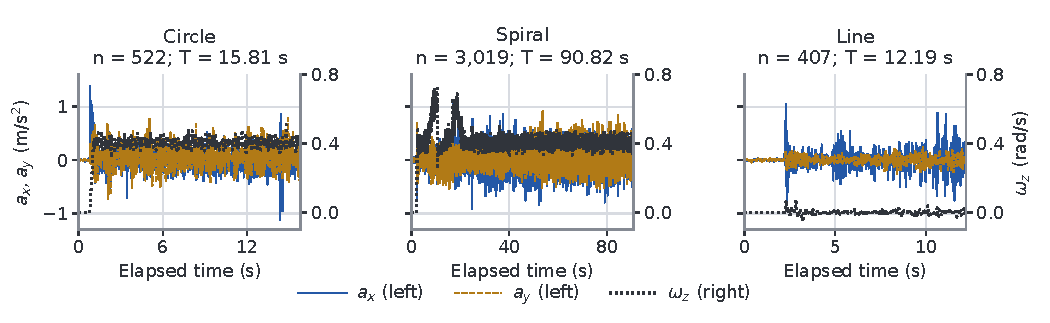
\includegraphics[width=\linewidth]{figures/imu_results.pdf}
\caption{Unsmoothed IMU samples on shared scales. Acceleration uses the left axes and angular rate the right; elapsed time starts at each file's first timestamp.}
\label{fig:imu}
\end{figure}

\clearpage
\textbf{Circle:} Mean $\omega_z$ is $0.402$~rad/s over 2--15~s of the 15.81~s recording, showing sustained turning after startup.

\textbf{Spiral:} Mean $\omega_z$ is $0.403$~rad/s over 25--90~s of the 90.82~s recording; larger early variations settle into steady turning.

\textbf{Line:} Mean $\omega_z$ is $5.4\times10^{-4}$~rad/s over 12.19~s, indicating little net rotation. The mean of $a_x$ is close to zero ($0.0017$~m/s$^2$), indicating that positive and negative readings largely balance over the recording.
